\subsection{CoDet-M4}
\label{section:CoDet-M4}
The main contribution of this work is the construction 
of a dataset derived from existing human-written code datasets, 
by generating synthetic code using six different LLMs. 
The authors then train several models on this dataset 
to evaluate their performance, 
demonstrating that their dataset can significantly improve 
the effectiveness of various code detection models.
The authors employ the following models as code generators:

\begin{itemize}
    \item \textbf{GPT-4o} \cite{openai_gpt4o_2024} : A proprietary model developed by OpenAI, selected to represent the state-of-the-art among large-scale, closed-source LLMs.
    
    \item \textbf{CodeLlama (7B)} \cite{roziere2023code} : An open-source model by Meta, specifically trained for code-related tasks. It is one of the most popular code-oriented language models.
    
    \item \textbf{Llama3.1 (8B)} \cite{meta_llama3_1_2024} : A more recent version of Meta’s Llama family. Although it is a general-purpose model, it exhibits strong performance in code generation.
    
    \item \textbf{CodeQwen 1.5 (7B)} \cite{qwen_codeqwen1.5_blog_2024} : An open-source model from Alibaba Cloud, also specialized in code, and part of the Qwen series.
    
    \item \textbf{Nxcode-orpo (7B)} \cite{ntqa_nxcode_dataloop_2024} : A fine-tuned variant of CodeQwen. The authors include it to evaluate the robustness of detectors against different fine-tuning strategies applied to the same base model (in this case, ORPO – Monolithic Preference Optimization).
\end{itemize}


\subsubsection*{Strengths}
\begin{itemize}
    \item The introduction of one of the most extensive and diverse datasets proposed for the task of LLM-generated code detection.
    \item The authors also construct an ``out-of-domain'' dataset, specifically designed to contain code with characteristics intentionally different from the main dataset {(\scriptsize\textit{Section 4.4:Out-of-Domain Experiment})}.
    \item The dataset includes code in three different programming languages, unlike other works that focus solely on Python {(\scriptsize\textit{Section 3.1: Data Collection})}.
\end{itemize}

\subsubsection*{Weaknesses}
\begin{itemize}
    \item Suspiciously high in-domain classification metrics, with F-scores exceeding 98\% {(\scriptsize\textit{Table 2})}.
    \item The prompts used to generate synthetic code vary depending on the source, potentially introducing an unintentional correlation between code types and the generation prompts {(\scriptsize\textit{Appendix F})}.
    \item Most of the LLMs used for code generation are lightweight models, with GPT-4o being the only large-scale LLM involved {(\scriptsize\textit{Section 3.2: Code Generation})}.
    \item Once the dataset is downloaded from the official portal on \href{https://huggingface.co/datasets/DaniilOr/CoDET-M4}{huggingface}, 
    several important intuitive reliability metrics are found to be missing:
    \begin{itemize}
        \item The declared train/validation/test split described in the paper is not 
        included; only the test set is provided. This makes 
        \textbf{reproducing their results more difficult}.
        \item Some significant \textbf{code-level features are missing}, 
        such as whether the code sample is class-based or function-based.
        \item The authors state in the paper that they plan to keep 
        updating the dataset, which may explain small discrepancies 
        in the number of code samples compared to what is reported. 
        For example, there are fewer GitHub samples than those 
        claimed in the original publication as shown 
        in Figure~\ref{fig:CoDet-M4_histogram_differences}
        The strange think is that the number of code not only 
        increased but 
        also decreased.
    \end{itemize}
    \item Focusing on the human code {(\scriptsize\textit{Section 3.1: Data Collection})}:
        \begin{itemize}
            \item \textbf{LeetCode corpora}: Pan et al. \cite{pan2024assessing} (5,069) and others (2,800) so the total should be: 7,869 
            but according to the paper table we should have 13,528 codes Figure~\ref{fig:CoDet-M4_histogram_differences} 
            \textit{(we don't know the source of half of the codes)}.
            \item \textbf{Code-Forces corpora}: the dataset has 103,792 codes but they are all
            solutions of only 2,523 problems from 
            a publicly available Kaggle dataset \cite{CodeforcesKaggle}.
            \item \textbf{GitHub corpora}: 135,566 codes from 
            CodeSearchNet \cite{husain2019codesearchnet} 
            and GitHub API in 2019 \textit{(code not up to date)}
        \end{itemize}
    \item Even if the dataset as a whole may appear fully balanced, 
    clear imbalances emerge when focusing solely on the human-written code:
            \begin{itemize}
            \item There is an imbalance in the number of code samples generated by 
            different LLMs (with relatively few generated by GPT models 
            Figure)
            \item LeetCode human-written code samples are significantly 
            fewer, meaning that many more generations were performed on 
            LeetCode problems compared to other corpora.
    \end{itemize}
\end{itemize}






\subsubsection*{Code Quality}
In order to preserve quality in the LLMs code source:
\begin{itemize}
    \item \textit{"For LLM-generated code, we filtered irrelevant responses and extracted code from the LLM output."}
    \item \textit{"After collecting the datasets, we \textbf{removed all comments and docstrings}."}
    \item \textit{"We also filtered codes based on length, excluding those below the 5th or above the 95th percentile in token count."}
    \item \textit{"Finally, we deduplicated the dataset to prevent potential code memorization."}
\end{itemize}


 %%%%%%%%%%%%%%%%%%%%%%%% IMGS
%\begin{figure}[ht]
%    \centering
%    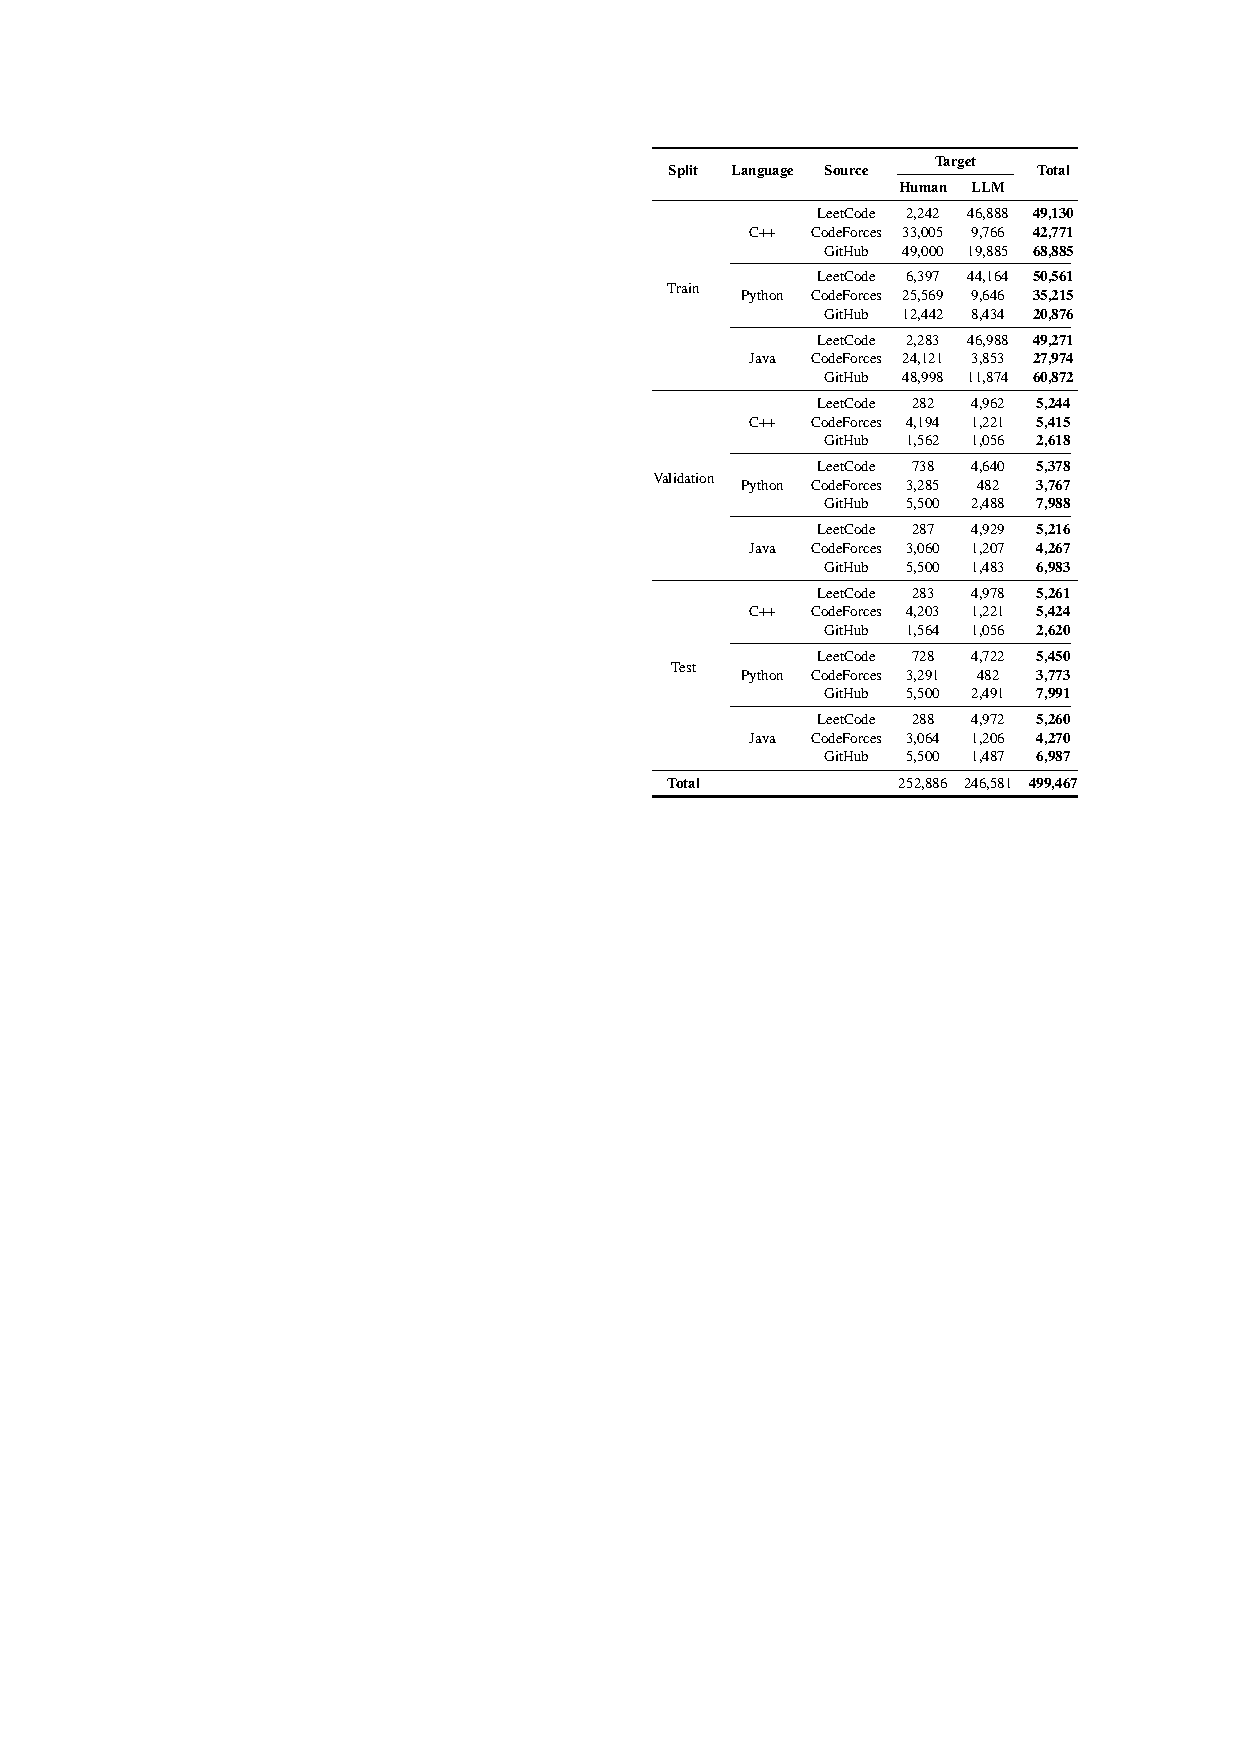
\includegraphics[width=0.5\textwidth]{img/CoDet-M4/tab1.pdf}
%    \caption{Table of dataset number of codes}
%    \label{fig:tabella-risultati}
%\end{figure}

%%%%%%%%%%%%%%%%%%%%%%%%%%%%%
\begin{figure}[h]
    \centering
    \begin{subfigure}[b]{0.45\textwidth}
        \centering
        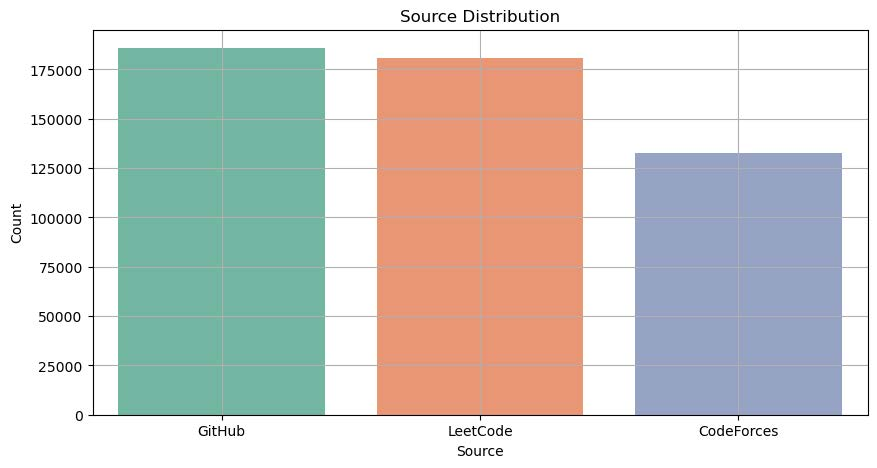
\includegraphics[width=\linewidth]{img/CoDet-M4/origianl_histogram_source_distribution.jpeg}
        \caption{Paper source distribution}
        \label{fig:immagine1}
    \end{subfigure}
    \hfill
    \begin{subfigure}[b]{0.45\textwidth}
        \centering
        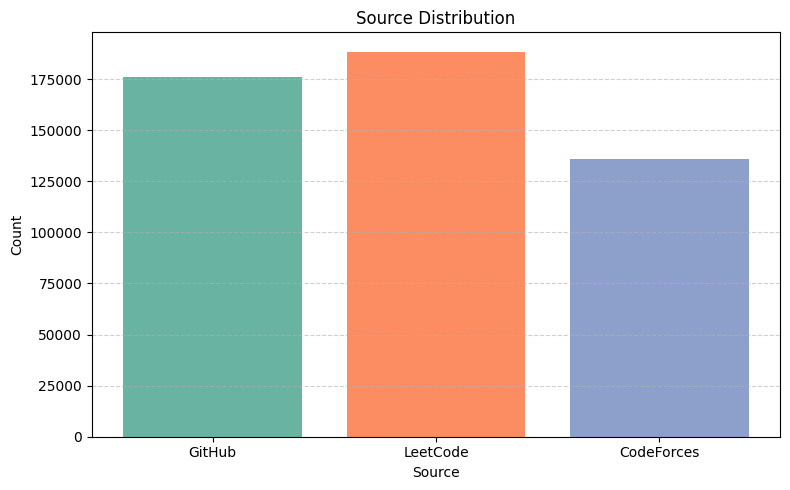
\includegraphics[width=\linewidth]{img/CoDet-M4/histogram_source_distribution_MY.png}
        \caption{Actual source distribution}
        \label{fig:immagine2}
    \end{subfigure}
    \caption{histogram differences}
    \label{fig:CoDet-M4_histogram_differences}
\end{figure}



%%%%%%%%%%%%%%%%%%%%%%%%%%%%%%%


%\begin{figure}[H]
%    \centering
%    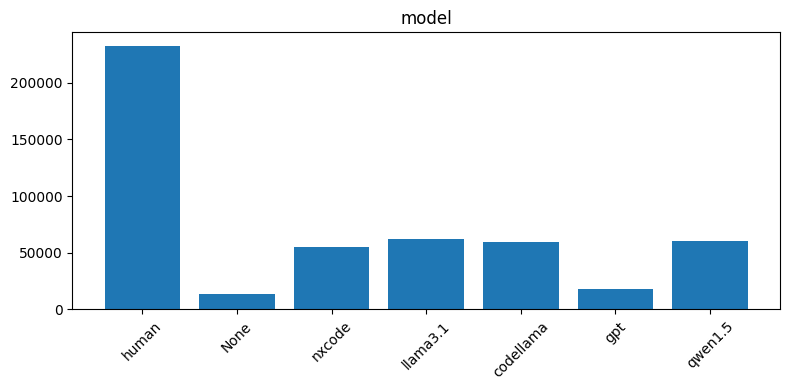
\includegraphics[width=0.6\textwidth]{img/CoDet-M4/models.png}
%    \caption{LLMs codes distribution}
%    \label{fig:LLMs_codes}
%\end{figure}

%\begin{figure}[H]
%    \centering
%    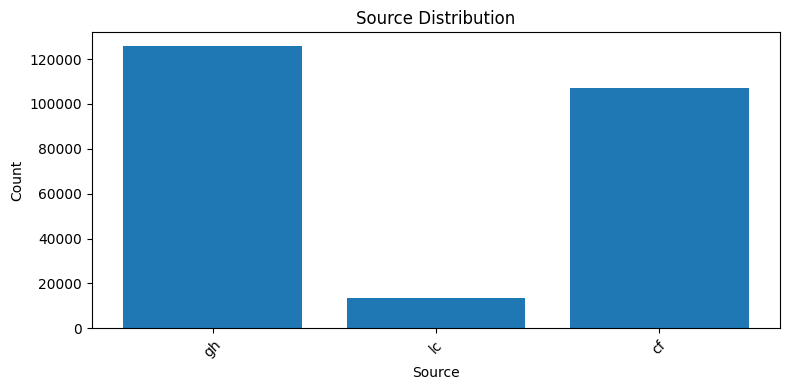
\includegraphics[width=0.6\textwidth]{img/CoDet-M4/lc_less.png}
%    \caption{human-written code distribution}
%    \label{fig:human-written_code_distribution}
%\end{figure}


%%%%%%%%%%%%%%%%%%%%%%%%%%%%%%%%%%%

\clearpage %%%%%%%%%%%%%%%%%%%%%%%%%%%%%
% TABLE

\subsubsection*{Final evaluation}

\expandafter\def\csname CoDetM4HumanCode\endcsname{246,221}
\expandafter\def\csname CoDetM4LLMCode\endcsname{254,331}
\expandafter\def\csname CoDetM4NumLLMs\endcsname{6 LLMs: \textit{(GPT-4o, CodeLlama 7B, Llama3.1 8B, CodeQwen 1.5 7B, Nxcode-orpo 7B )}}
\expandafter\def\csname CoDetM4LLMDiversity\endcsname{3 different source models: \textit{(GPT-4o, CodeLlama, CodeQwen) }}
\expandafter\def\csname CoDetM4CurrentUse\endcsname{Average LLMs release date: 2024}
\expandafter\def\csname CoDetM4Languages\endcsname{Python, Java, C++}
\expandafter\def\csname CoDetM4CodeTypes\endcsname{Functional, Object-Oriented \textit{(missing information in the dataset)}}
\expandafter\def\csname CoDetM4CodeSize\endcsname{1\textsuperscript{st} percentile: 42 words,\newline 3\textsuperscript{rd} percentile: 68 words}
\expandafter\def\csname CoDetM4CodeContext\endcsname{Mixed (competitive and open-source)}
\expandafter\def\csname CoDetM4Prompts\endcsname{Provided (different between LLMs)}
\expandafter\def\csname CoDetM4Sources\endcsname{GitHub, Codeforces \cite{CodeforcesKaggle}, Pan et al. \cite{pan2024assessing}}
\expandafter\def\csname CoDetM4CodeQuality\endcsname{Comment removal, Duplicate code removal}
\expandafter\def\csname CoDetM4Reliability\endcsname{Low, missing or inconsistent information}


\evaluationTable{CoDetM4}


Despite being a very interesting dataset, 
especially due to the large amount of available code, 
it proves to be unreliable both because of the authors' 
lack of precision and due to some of its intrinsic 
characteristics, such as an unusual data imbalance. 
While it is not a dataset to be entirely discarded, 
its use must certainly be carefully evaluated.